%!TEX root = cscw2018-comic.tex
\section{Method}
\label{sec:Method}

In this section, we discuss our methodology for evaluating the effectiveness of comic form messages. First we discuss the example messages used with positive and negative framing. Then, we show how we algorithmically synthesize the comic messages. Then we discuss how we instantiated the study on Amazon Mechanical Turk, followed by a discussion of how we evolved our experiment design based on Turker feedback. We conclude this section with a discussion of how we identified potential subjects on Amazon Mechanical Turk.

\subsection{Composing Persuasive Messages in Plain Text}
We use simple text messages with a goal to persuade subjects to engage in more physical activity. We chose this topic as we felt that health is a topic to which our experimental subjects could relate. We kept a single topic to ensure that we don't have any experimental confounds due to different topics.

% Aligned with the idea of memorability, the main theme of all persuasive messages and simple, persuading the target persuadee to engage more physical activity. The main reasons to choose this topics are 1) As a basic daily activity everyone has the need to exercise. 2) People can easily understand the message and relate to themselves. 3) Engaging more exercise is mostly based on audience own willingness instead of any other subjective resources.

We constructed messages based on the idea of social proof~\cite{goldstein2008room}, where the messages emphasized the relationship between the subject and her group of friends. We created two sets of messages that either framed from a positive standpoint or a negative standpoint \cite{tversky1981framing}.

The followings messages were presented in our study.
\textit{Positive framed persuasive messages:}
\begin{enumerate}
 \item In the past week, you spent more time at the gym than did 65\% of your friends
 \item Congrats! You have reached your goal of exercising three times a week.
 \item Over the past month, you exercised more than did 90\% of your friends.
 \item Your exercise activity is in the top 20\% of all your friends.
 \item Over the past three weeks, you went to the gym more often than 60\% of your friends did.
\end{enumerate}\par
\textit{Negative framed persuasive messages:}
\begin{enumerate}
 \item	In the past week, you spent less time at the gym than did 65\% of your friends
 \item  Oh! You did not reach your goal of exercising three times a week.
 \item	Over the past month, you exercised less than did 90\% of your friends.
 \item	Your exercise activity is in the bottom 20\% of all your friends.
 \item	Over the past three weeks, you went to the gym less often than 60\% of your friends did.
\end{enumerate}

\subsection{Generating Comics}
In this study, we use a common template to generate comic messages that includes two characters in a conversation and the scenario is `One day, your friend has something to tell you.'

We developed an comic generator that based on Comix I/O, an open source project that creates comics with stick figures using HTML markup ~\cite{cmx.io}. We further developed the existing Comix I/O build with Canvas and rough.js \cite{canvasjs,rough.js}. The resulting generator takes in as input the characters gesture, inter-character spacing and the intensity of the background and allows us to create the comic representation of a persuasive message in XKCD style~\cite{munroe2009xkcd}.

\begin{figure}[b]
 \centering
 \begin{tabular}{cc}
  \subfloat[Three levels of gesture intensity for positive framed messages from neutral to the happiest]{\label{figur:1a}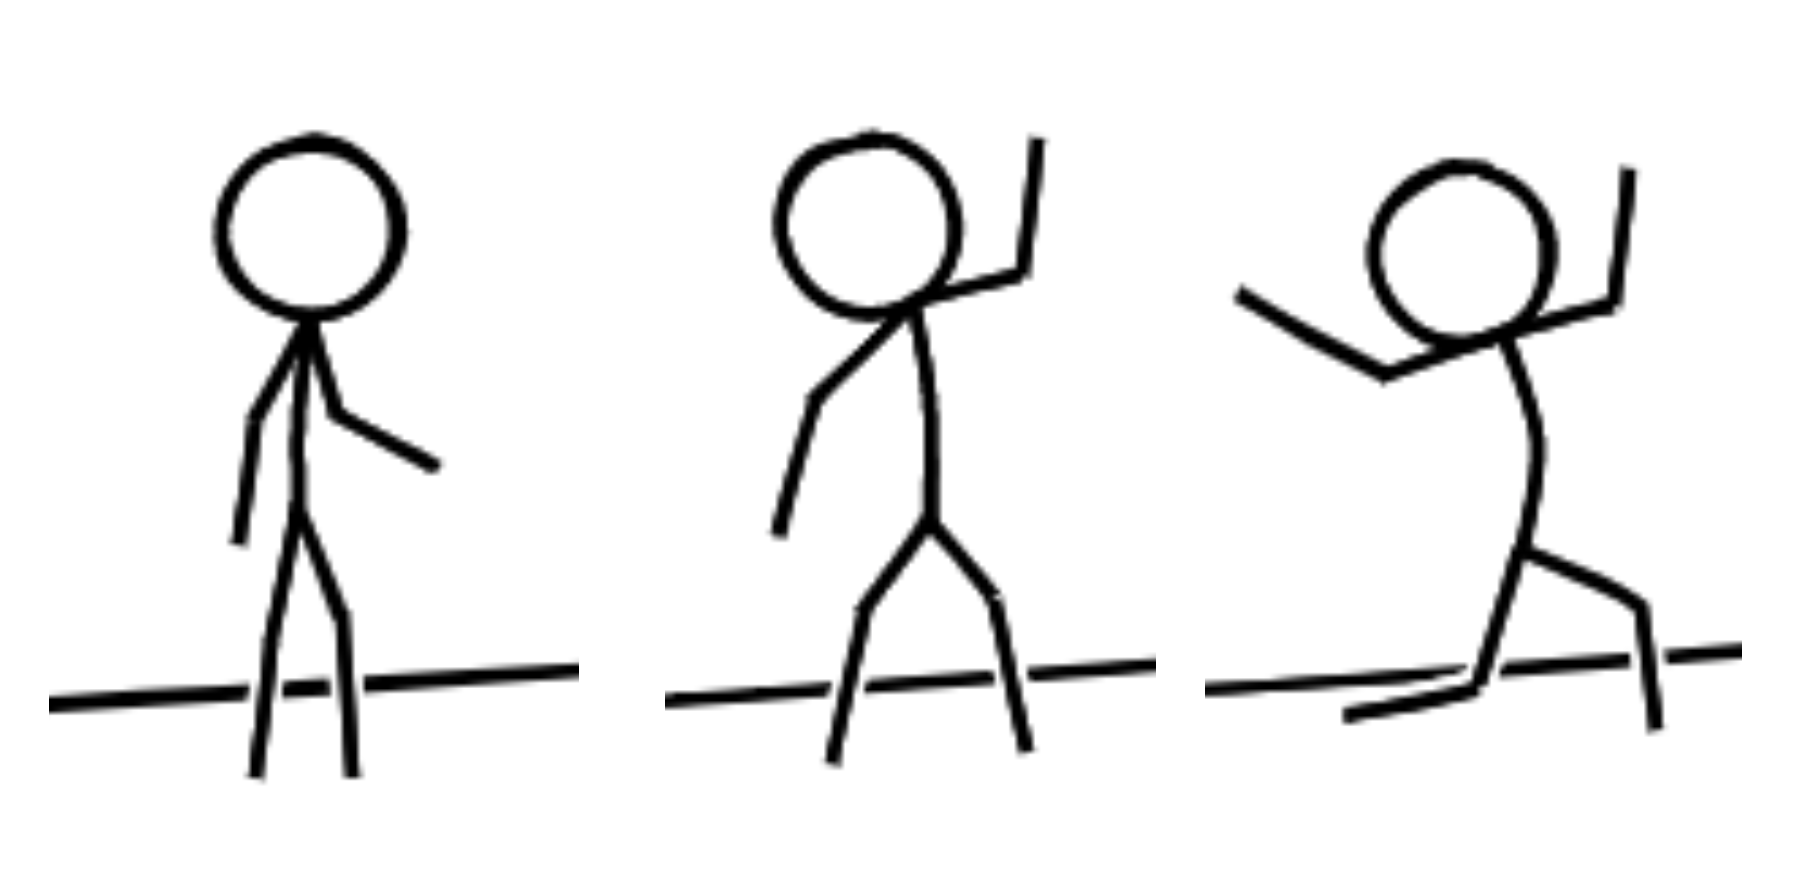
\includegraphics[width = 0.4\columnwidth]{figures/pos_figures}} &
  \subfloat[Three levels of gesture intensity for negative framed messages from neutral to the most frustrated ]{\label{figur:1b}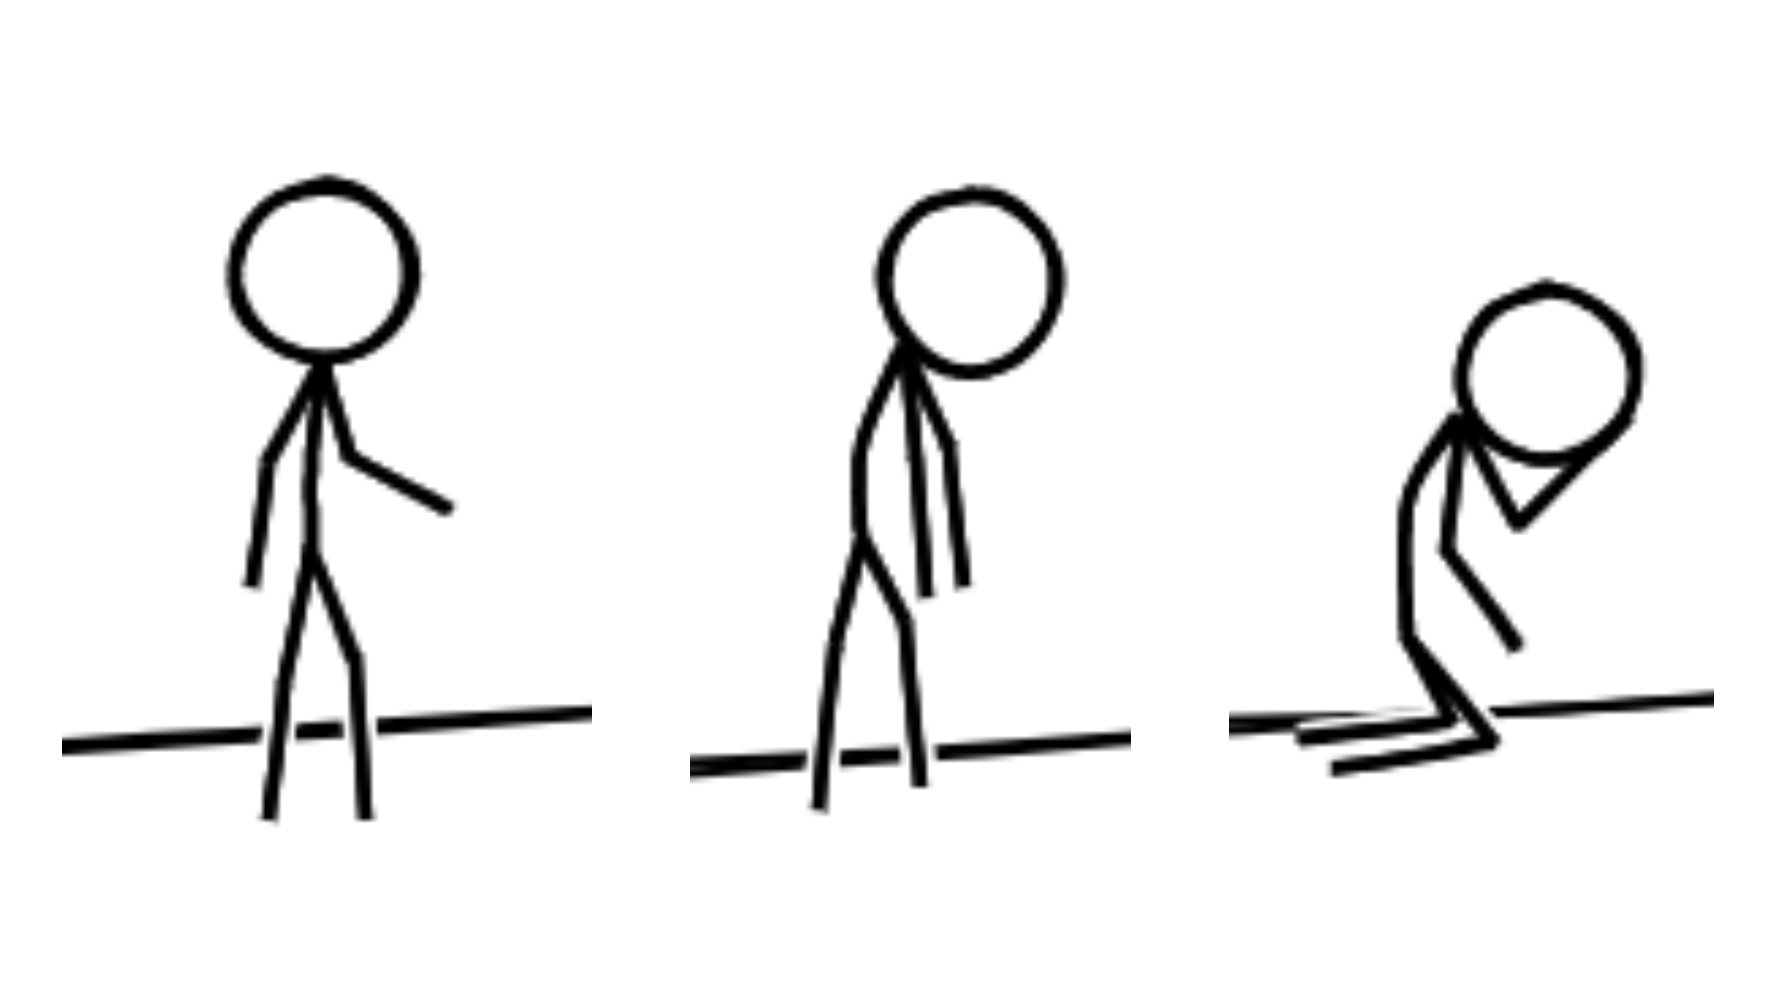
\includegraphics[width = 0.4 \columnwidth]{figures/neg_figures}}\\
 \end{tabular}
 \caption{Different character gestures to communicate various levels of emotional intensity}
 \label{figur:figures}
\end{figure}

\begin{figure}[t]
 \centering
 \begin{tabular}{ccc}
  \subfloat[Close Friends]{\label{figur:3a}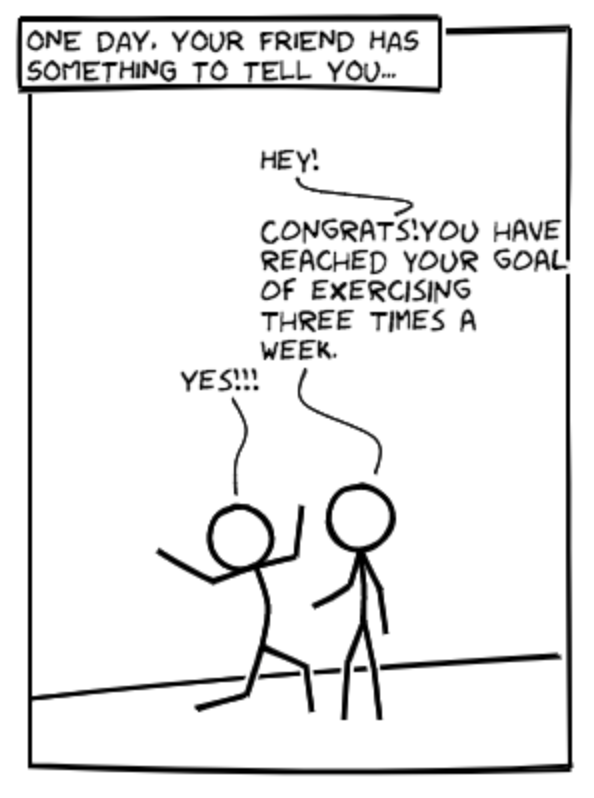
\includegraphics[width = 0.27\columnwidth]{figures/d0}} &
  \subfloat[Friends]{\label{figur:3b}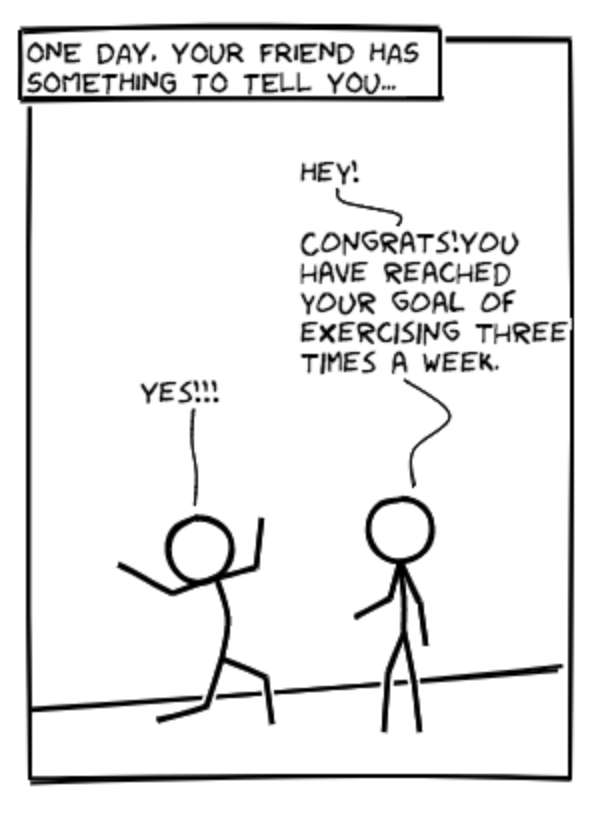
\includegraphics[width = 0.27 \columnwidth]{figures/d1}}      &
  \subfloat[Acquaintance]{\label{figur:3c}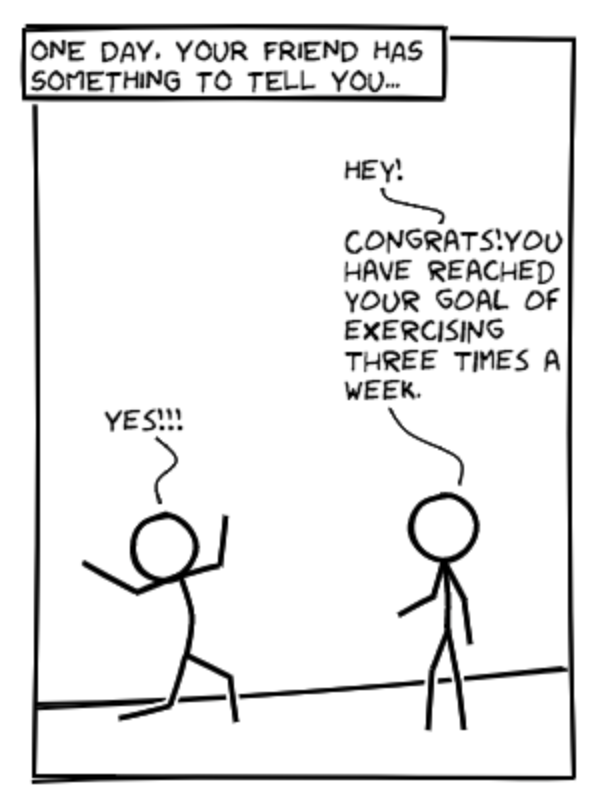
\includegraphics[width = 0.27 \columnwidth]{figures/d2}}\\
 \end{tabular}
 \caption{Different distance to communicate various levels of relationship closeness}
 \label{figur:distance}
\end{figure}

To make a fair comparison between plain text representation and the comic form, the content of text bubble is the same in both conditions. We discuss generation of elements of gesture, distance between characters and shading below.

\begin{description}
 \item[Gesture]: For each gesture, we created the gesture library in a JSON format with two main categories: positive and negative corresponding to how the original message is framed, each with three levels of emotional intensity see Figure~\ref{figur:figures}.
 \item[Inter-character distance]: For the distance between two characters, we have three levels of variance from close to medium separation to large separation. The three levels of distance represents the relationship between to characters as close friends, friends, and acquaintances; see Figure~\ref{figur:distance}.
 \item[Shading]: For the background shading, we have a total of three levels from white to dark grey. Each level represents a level of emotional intensity, white as lowest, see Figure~\ref{figur:shading}.
\end{description}






\begin{figure}[]
 \centering
 \begin{tabular}{ccc}
  \subfloat[Lowest]{\label{figur:4a}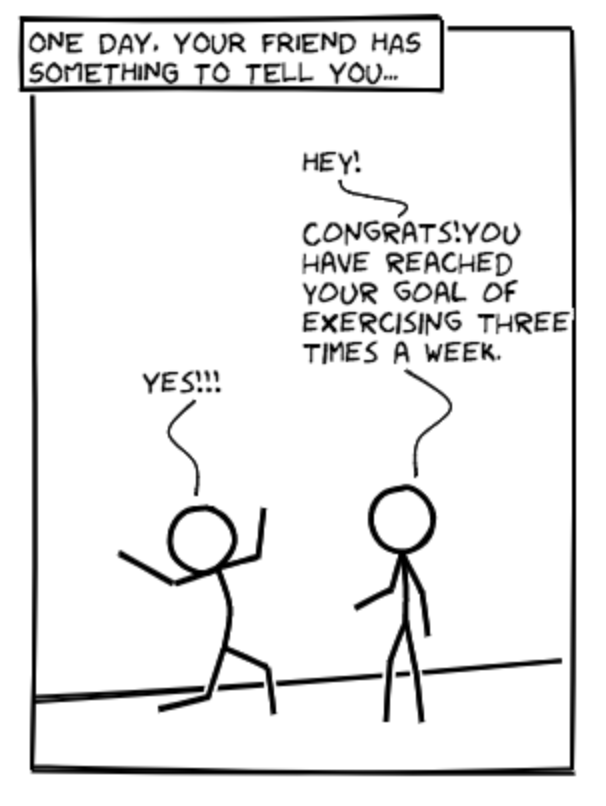
\includegraphics[width = 0.27\columnwidth]{figures/s0}}    &
  \subfloat[Moderate]{\label{figur:4b}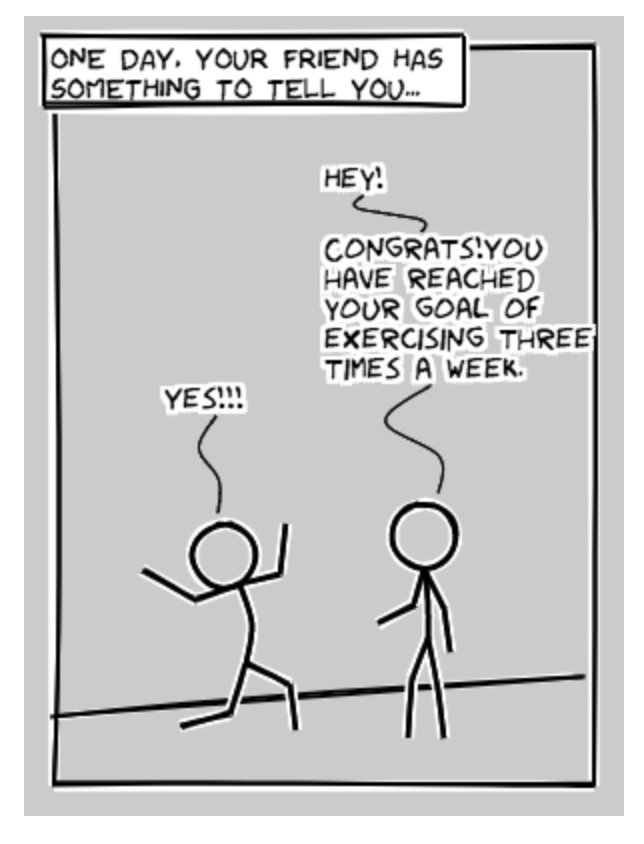
\includegraphics[width = 0.27 \columnwidth]{figures/s1}} &
  \subfloat[Intense]{\label{figur:4c}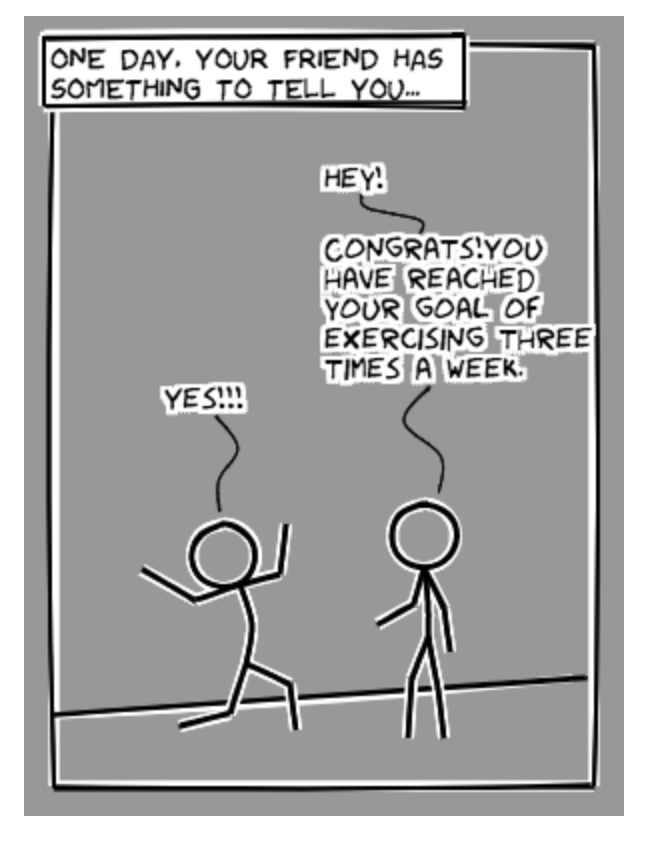
\includegraphics[width = 0.27 \columnwidth]{figures/s2}}\\
 \end{tabular}
 \caption{Different background to communicate various levels of emotional intensity}
 \label{figur:shading}
\end{figure}

In total, for each message we have a total of 54 variations in terms of character gesture, inter-character, background shading, and message framing. In this study, 270 comics was created corresponding to 5 plain text messages, e.g. Figure~\ref{figur:distance}, Figure~\ref{figur:shading}.

\subsection{Pilot Study Design}
To answer our research questions, we designed and after IRB approval, conducted a pilot between-subject online study on Amazon Mechanical Turk.

\textit{Experiment Procedure.} Once participant consented to join our study, they were randomly assigned to two conditions 1) Positive message condition where all persuasive messages are framed in a positive way and 2) Negative condition where all persuasive messages are framed in a negative way. In both conditions, participants will see a total of five persuasive messages in both plain-text representation and comic representation shown side by side. Then, the participant rates which representation of the message is perceived as more persuasive on a 7-item Likert scale.

\textit{Display Order.} To mitigate any potential bias toward the display order of the plain-text representation and comic representation we randomize the display order. Both plain-text representation and comic-style representation have equal chance to show on the left side.

\textit{Attention Checker.} To control the data quality, we embedded two attention checkers in the study. The first one appears after the third comparison and the second one shows up after the last comparison. Both attention checkers asked subjects to choose a comic that matches a simple description, e.g. ``Which of the following comics has two characters?''

\textit{Rating Scale Design.} The 7-item Likert scale ranges from -3 (left) to 3 (right) where 0 means neutral. The direction of the scale flips corresponding to the position of the comic and plain text, see the right part of Figure~\ref{fig:change}.


\subsection{Results from Pilot Study}
We received total of 10 responses in 5 hours. 5 of 10 participants reported through study feedback that the scale is confusing. Three of them reported the flipped scale makes them spend more time on figuring out which side represents which. One participant said ``When I am answering my last question, I suddenly noticed the scale is different. I noticed the order of text and graph is changing but never notice the scale is changing as well. That's really confusing!!''

Based on the feedback from our pilot test, we iterated our study design. In the final design, we fixed the order of the rating scale. However, since the order is fixed, potential demand characteristics may be introduced by the scale~\cite{orne1962social}. To minimize potential bias we added another layer of randomness in our final design. The direction of the scale no longer changes respect to the position of the messages, but the direction of the scale is randomly assigned for each participant. Also, we replaced the numbers on the scale by text as neutral, slightly persuasive, text/comics is more persuasive and strongly persuasive. Finally, three out of 10 participants told us the text representation of the message was hard to read. Therefore, we adjusted the size of the comic and text to make sure both of them have similar readability.

The left side of Figure~\ref{fig:change} shows the final design. Another round of pilot study with another 10 participants showed the newer design successfully addressed the problems in the old design and we encountered no new problems.

\begin{figure}
 \centering
 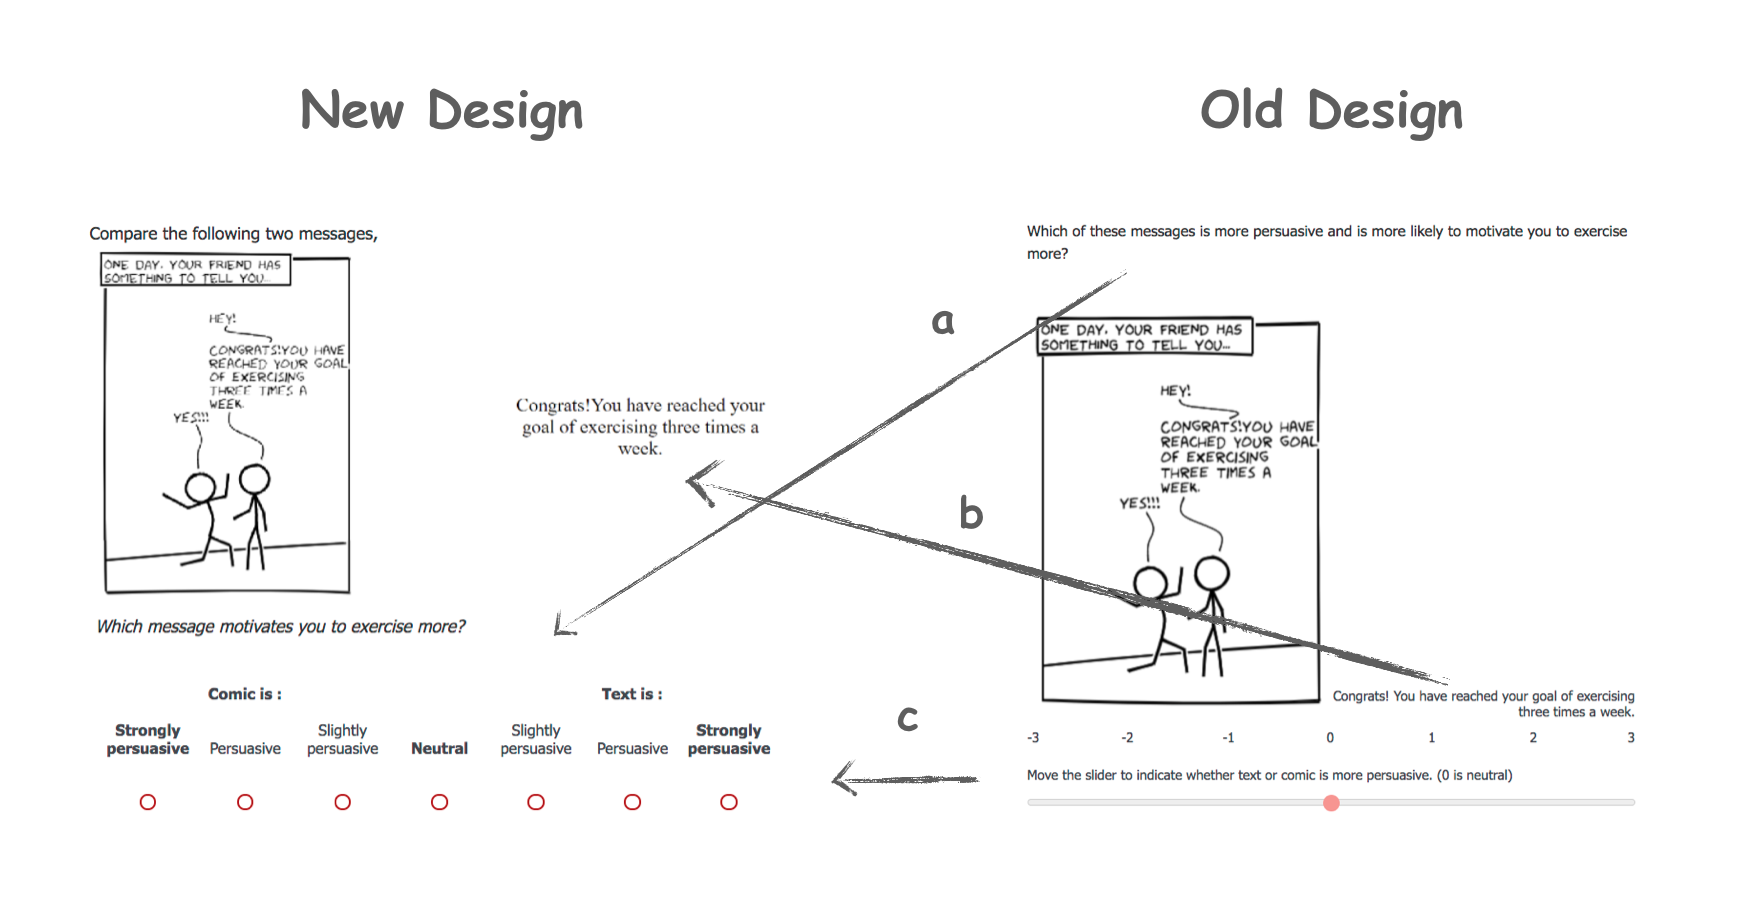
\includegraphics[width=0.95\columnwidth]{figures/change}
 \caption{Design of the task before and after the pilot study. A. Change the position of the question to makes the question more clear. B. Adjust the position and the size of the text message to improve readability. C. Improve the rating scale to make it easy to interpreted.}
 \label{fig:change}
\end{figure}


\subsection{Participants}
We published our HITs on Amazon Mechanical Turk titled with ``A short survey about your exercise motivation.'' The price tag for each HIT was \$8/hr, and the workers would get these rewards regardless of their performance. The threshold for participant to join our study was a 95\% Approval Rate. On the HIT page, participants would see a link to our experiment site and a text input box for them to enter a six-digit completion code. A worker who repeats the task will be rejected as we instructed in the task description.
